\documentclass[10pt,a4paper]{article}
\usepackage[margin=2.2cm]{geometry}
\usepackage{fontspec}
\usepackage{amsmath}
\usepackage{booktabs}
\usepackage{longtable}
\usepackage{graphicx}
\usepackage{float}
\usepackage{xcolor}
\usepackage{enumitem}
\usepackage[hidelinks]{hyperref}
\setlist{nosep, leftmargin=1.4em}
\setlength{\parskip}{0.45em}
\setlength{\parindent}{0pt}
\graphicspath{{results/figures/}}
\newcommand{\file}[1]{\texttt{\small #1}}
\newcommand{\reasoning}[1]{\textit{(Reasoning, not proven by the data:)} #1}

\title{IRWA project, Part 3: Ranking and Filtering}
\date{}
\begin{document}
\maketitle
\vspace{-3em}

\section*{Setup}

Code and results: \url{https://github.com/Vagaroto/RIAW-Presentaci-nFinal} (folder \file{Part3/}).
\file{Base.py} holds the index, the conjunctive search and the evaluation; \file{Scoring.py} the rankings;
\file{Figures.py} the evidence and figures of this report. Every number below cites the CSV file in
\file{Part3/results/} it comes from. Run \file{py -m part3.Scoring}, then \file{py -m part3.Figures} and
\file{py -m part3.build\_report} from the repository root.

\textbf{Pipeline.} A query goes through the same preprocessing as the products (Part 1: normalization,
stop words, Snowball stemming). The candidates are the products that contain \emph{every} query term (AND),
the intersection of the postings lists. Only then a ranking orders them. All rankings share one signature,
\file{ranking(query\_terms, candidates, prep)}, so they rank exactly the same candidate sets and differ
only in the order. 

\textbf{Implementation choice.} The preprocessing is imported from Part 1, and the queries, labels and
metrics from Part 2. The index, the search and the evaluation loop were rewritten in \file{Base.py}
instead of reused. In Part 2 the functions split the work unevenly: the search preprocessed the query and
called TF-IDF directly, TF-IDF scored every product and left the AND filter to the caller, and BM25 took
different arguments and recomputed the product lengths on every call. Here the index statistics (idf,
norms, lengths) are computed once in \file{prepare}, the search only applies the AND filter, and every
ranking only orders the candidates it receives, with the same inputs. Any ranking can then be passed to
\file{search} and \file{evaluate} unchanged, which is what lets us compare five rankings on exactly the
same candidates.

\textbf{Missing labels lower the metrics of the new rankings.} Only the products of
\file{validation\_labels.csv} and the top 20 of the Part 2 ranking (\file{Part2/test\_labels.csv}) have a
label, and an unlabeled product counts as not relevant. A ranking that returns products the Part 2 ranking
did not is therefore penalized even when those products are relevant. All metrics in this report are
read with that in mind (Section 1.5, Table~\ref{tab:p10}); we did not label the extra results, since the
assignment does not ask for it.

\textbf{Queries.} The two validation queries and the five test queries of Part 2 (\file{queries.csv}):

\begin{table}[H]
\centering\small
\begin{tabular}{r l r}
\toprule
\# & Query & AND matches \\
\midrule
1 & women full sleeve sweatshirt cotton & 500 \\
2 & men slim jeans blue & 222 \\
3 & men polo t-shirt & 1,451 \\
4 & men round neck half sleeve cotton t-shirt & 2,046 \\
5 & reebok men t-shirt & 72 \\
6 & men raincoat & 23 \\
7 & white linen shirt & 24 \\
\bottomrule
\end{tabular}
\end{table}

\section{Three ways of ranking}

Notation: $\mathrm{tf}(t,d)$ is the number of times term $t$ appears in product $d$,
$\mathrm{idf}(t)=\ln(N/\mathrm{df}(t))$ with $N=28{,}080$, $|d|$ the length of $d$ in tokens and
$\overline{|d|}=52.1$ the mean length (\file{corpus\_numeric.csv}).

\subsection{TF-IDF + cosine similarity (\file{tf\_idf\_cosine})}

Each text is a vector of weights $w(t,d)=\mathrm{tf}(t,d)\cdot\mathrm{idf}(t)$ (the same weights as Part 2),
and the score is the cosine between the query vector $q$ and the product vector $d$:
\[
\cos(q,d)=\frac{\sum_{t\in q} w(t,q)\,w(t,d)}{\lVert q\rVert\,\lVert d\rVert}.
\]
$\lVert d\rVert$ is computed once over \emph{all} the terms of the product. $\lVert q\rVert$ is the same
for every candidate, so it is dropped: it does not change the order (this is why the scores in
\file{rankings\_top10.csv} are above 1).

\subsection{BM25 (\file{bm25})}

\[
\mathrm{BM25}(q,d)=\sum_{t\in q}\mathrm{idf}(t)\,
\frac{(k_1+1)\,\mathrm{tf}(t,d)}{k_1\left((1-b)+b\,\frac{|d|}{\overline{|d|}}\right)+\mathrm{tf}(t,d)},
\qquad k_1=1.4,\; b=0.25.
\]
$k_1$ makes the contribution of a term saturate as its frequency grows; $b$ sets how much a product longer
than the mean is penalized. We kept the values of Part 2 and did not tune them on the labels, which
would make the evaluation optimistic. $b=0.25$ is below the usual $0.75$, so the length penalty is mild.

\subsection{How the two rankings differ}

\textbf{They return different products.} On average the top 10 of TF-IDF cosine and of BM25 share only
2.7 products (Figure~\ref{fig:overlap}, \file{top10\_overlap.csv}). Both see the same candidates; the
difference is entirely in how frequency and length are combined.

\begin{figure}[H]
\centering
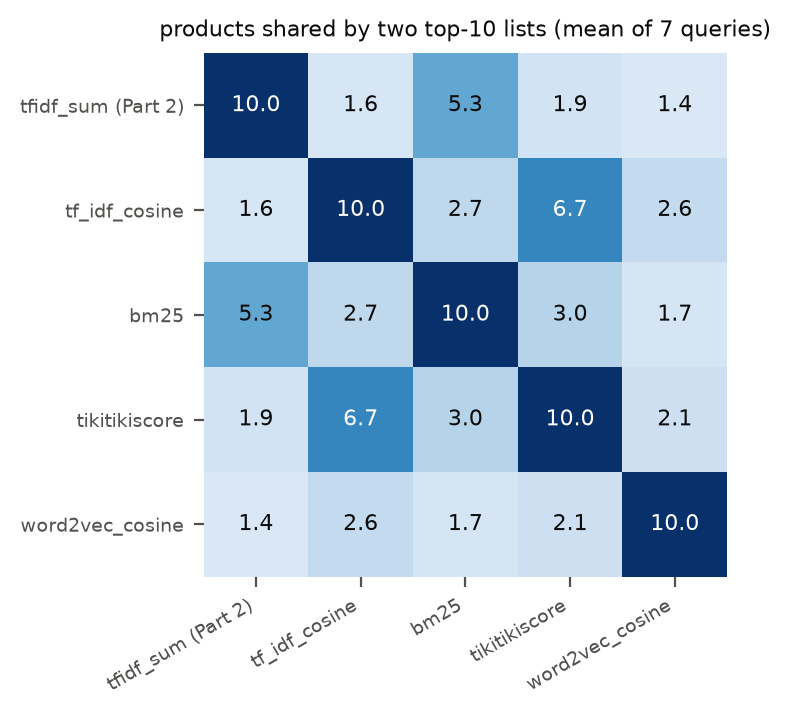
\includegraphics[width=0.55\textwidth]{overlap.png}
\caption{Mean number of products shared by the top 10 of two rankings, over the 7 queries. Source:
\file{top10\_overlap.csv}.}
\label{fig:overlap}
\end{figure}

\textbf{Cosine prefers short products, BM25 does not.} Figure~\ref{fig:lengths} (\file{top10\_profile.csv})
shows the mean length of the top 10 of each ranking. For all seven queries the cosine top 10 is
\emph{shorter} than the average product (31 to 45 tokens against 52.1). Dividing by $\lVert d\rVert$
penalizes every extra word, so a short product whose few words include the query wins. BM25 top 10s are
between 49 and 99 tokens: with $b=0.25$ the length is only lightly penalized, and the saturation through
$k_1$ is what stops long, repetitive texts from winning. The unnormalized sum of Part 2 is the extreme
case (up to 203 tokens on query 3).

\begin{figure}[H]
\centering
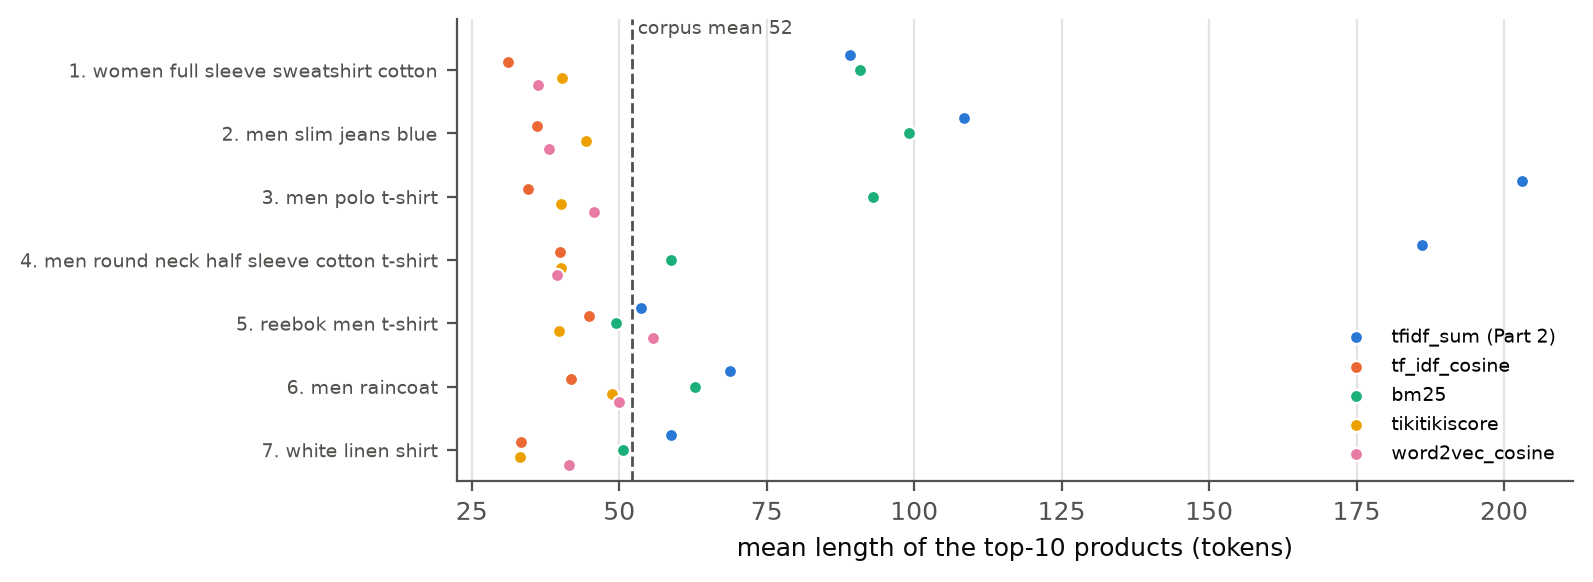
\includegraphics[width=\textwidth]{lengths.png}
\caption{Mean length of the top-10 products of each ranking, per query. Dashed line: mean length of the
28,080 products. Source: \file{top10\_profile.csv}, \file{corpus\_numeric.csv}.}
\label{fig:lengths}
\end{figure}

\textbf{An example, query 3 \texttt{men polo t-shirt}} (stemmed terms \texttt{men}, \texttt{polo},
\texttt{tshirt}; first result of each ranking, \file{first\_results.csv}):

\begin{table}[H]
\centering\small
\begin{tabular}{l r l l}
\toprule
Ranking & Length & tf (men, polo, tshirt) & Title \\
\midrule
TF-IDF sum (Part 2) & 623 & 22, 8, 60 & Color Block Men V Neck Dark Blue T-Shirt \\
TF-IDF cosine       & 28  & 2, 3, 2   & Solid Men Polo Neck Grey T-Shirt \\
BM25                & 72  & 4, 6, 7   & Solid Men Polo Neck Maroon T-Shirt \\
\bottomrule
\end{tabular}
\end{table}

Without normalization, a 623-token description that repeats \texttt{tshirt} 60 times wins although the
product is a V-neck. Cosine picks a 28-token polo shirt; BM25 a 72-token one, because 6 or 7 occurrences
add more than they cost in length.

Table~\ref{tab:proscons} sums up the pros and cons.

\begin{table}[htb]
\centering\small
\caption{Pros and cons of TF-IDF cosine and BM25.}
\label{tab:proscons}
\begin{tabular}{p{0.12\textwidth} p{0.39\textwidth} p{0.39\textwidth}}
\toprule
 & Pros & Cons \\
\midrule
TF-IDF\newline cosine &
No parameters. Normalizing by $\lVert d\rVert$ removes the advantage of long, keyword-stuffed texts
(query 3). Standard and easy to explain. &
Over-corrects: favours short products, which may have just a title and a few details. Linear tf: a term
repeated many times still counts in full. $\lVert d\rVert$ depends on terms that have nothing to do with
the query. \\
\addlinespace
BM25 &
Saturating tf ($k_1$): repeating a term has a decreasing effect. Length normalization is tunable ($b$),
relative to the mean length. Strong standard baseline in IR. &
Two parameters to set, ideally on judged data we do not have enough of. With a small $b$ long products
are still preferred (Figure~\ref{fig:lengths}). Scores are not bounded, so they are not comparable
across queries (the same holds for our cosine, which drops $\lVert q\rVert$). \\
\bottomrule
\end{tabular}
\end{table}

\subsection{Our score (\file{tikitikiscore})}

\[
\mathrm{score}(q,d)=\cos(q,d)\times\underbrace{\frac{\mathrm{rating}(d)}{5}}_{0.7\text{ if no rating}}
\times\underbrace{\begin{cases}0.5 & \text{out of stock}\\ 1 & \text{otherwise}\end{cases}}_{\text{stock}}
\]

The text match (TF-IDF cosine) decides whether a product is about the query; two numeric fields then say
whether it is a good result \emph{to show}:
\begin{itemize}
\item \textbf{Rating.} Among products that match equally well, a user prefers one that buyers rated well.
  A product without a rating (2,261 products, 8.1\%, \file{corpus\_numeric.csv}) gets 0.7, the factor of
  a 3.5 rating, close to the mean rating of 3.63: unknown is treated as roughly average, not as bad, so
  new products are not buried.
\item \textbf{Stock.} An out-of-stock product (1,644 products, 5.9\%) cannot be bought, but it still
  answers the query, so it is halved, not removed.
\item \textbf{Not used:} price and discount. A cheaper or more discounted product is not more relevant to
  the query; which one is better depends on the user, so we left them for filters rather than the score.
\end{itemize}

\textbf{Effect} (\file{top10\_profile.csv}, \file{top10\_overlap.csv}, \file{score\_effect.csv}). It keeps 6.7 of the 10 cosine
results on average, so the text match still dominates. Over the seven queries, the cosine top 10s contain
6 out-of-stock and 4 unrated products; ours contain 0 and 1. For \texttt{men slim jeans blue} the mean
rating of the top 10 goes from 2.76 to 4.07: the eight products that leave the top 10 are \emph{Slim Men
Blue Jeans} and \emph{Super Skinny Men Blue Jeans} rated 2.5 or out of stock.

\textbf{Pros.} Uses information the text does not have; simple and readable (each factor can be
explained to a user); only reorders, it never removes a product. \textbf{Cons.} The factors 0.7 and 0.5
are chosen by reasoning, not fitted (there are too few labels to fit them without inflating the
evaluation). The rating ignores the number of reviews: a 5.0 from one buyer beats a 4.4 from thousands.
It multiplies the cosine, so it inherits its preference for short products.
\reasoning{a well-rated product is more likely to satisfy the user, but the labels judge relevance to the
query, not quality, so they cannot show this benefit.}

\subsection{Evaluation and its limit}

Figure~\ref{fig:metrics} (left, \file{evaluation.csv}) gives the mean of P@10, NDCG@10, MAP and MRR over the
seven labeled queries. Taken at face value, the Part 2 ranking is best (P@10 0.543 against 0.400 for
cosine and BM25 and 0.371 for our score). \textbf{This comparison is biased.} The labels of the test
queries were made from the top 20 of the Part 2 ranking, and a product without a label counts as not
relevant. The right panel (\file{top10\_judgements.csv}) splits the top-10 results: the new rankings
return mostly products nobody judged (40 of 70 for cosine), and very few judged \emph{not} relevant
(2 for cosine, 3 for BM25), while the Part 2 ranking has 14.

\begin{figure}[H]
\centering
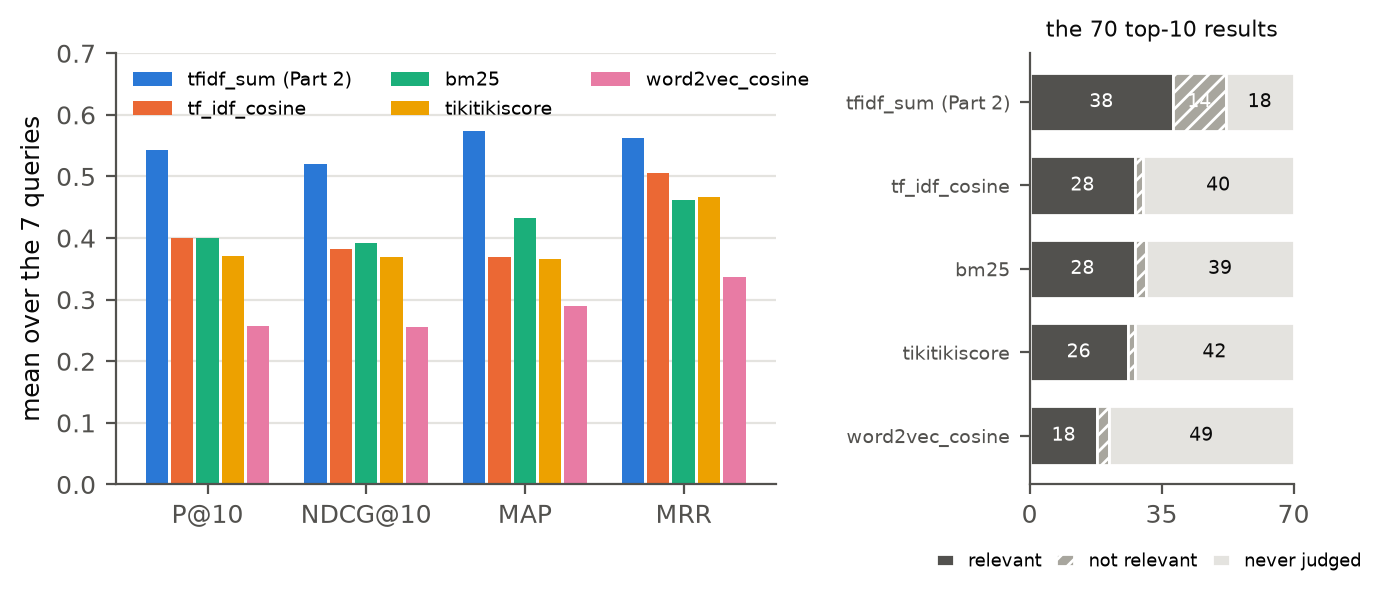
\includegraphics[width=\textwidth]{metrics.png}
\caption{Left: mean metrics over the 7 queries. Right: the 70 top-10 results of each ranking (7 queries
$\times$ 10) by label. Sources: \file{evaluation.csv}, \file{top10\_judgements.csv}.}
\label{fig:metrics}
\end{figure}

Precision among the \emph{judged} results only is 38/52 = 0.73 for Part 2, 28/30 = 0.93 for cosine,
28/31 = 0.90 for BM25, 26/28 = 0.93 for our score and 18/21 = 0.86 for word2vec. The zeros of P@10 on
queries 3 and 4 for cosine and BM25 are all unjudged products, and their titles are what the query asks
for (\emph{Solid Men Polo Neck Grey T-Shirt}, \emph{Solid Men Round Neck Beige T-Shirt}). We did not
label the extra results, since the assignment does not require it, so we draw no conclusion on which
ranking is better from these metrics; the comparison above rests on the orderings themselves.

\begin{table}[H]
\centering\small
\begin{tabular}{r l l l l l l}
\toprule
\# & Query & Sum (P2) & Cosine & BM25 & Ours & word2vec \\
\midrule
1 & women full sleeve sweatshirt cotton & 0.2 (8) & 0.0 (10) & 0.1 (9) & 0.1 (9) & 0.0 (10) \\
2 & men slim jeans blue                 & 0.0 (10) & 0.2 (8) & 0.0 (10) & 0.1 (9) & 0.2 (8) \\
3 & men polo t-shirt                    & 0.9 (0) & 0.0 (10) & 0.0 (10) & 0.0 (10) & 0.0 (10) \\
4 & men round neck half sleeve cotton t-shirt & 0.0 (0) & 0.0 (10) & 0.0 (10) & 0.0 (10) & 0.0 (10) \\
5 & reebok men t-shirt                  & 1.0 (0) & 0.9 (1) & 1.0 (0) & 0.8 (2) & 0.0 (10) \\
6 & men raincoat                        & 1.0 (0) & 0.9 (1) & 1.0 (0) & 0.9 (1) & 0.9 (1) \\
7 & white linen shirt                   & 0.7 (0) & 0.8 (0) & 0.7 (0) & 0.7 (1) & 0.7 (0) \\
\midrule
 & Mean P@10 & 0.543 & 0.400 & 0.400 & 0.371 & 0.257 \\
 & Unjudged in the top 10 & 18 & 40 & 39 & 42 & 49 \\
\bottomrule
\end{tabular}
\caption{P@10 per query; in brackets, how many of the 10 results were never judged and therefore
count as not relevant (\file{evaluation.csv}, \file{top10\_judgements.csv}). Every 0.0 of the new
rankings on queries 3 and 4 comes from 10 unjudged products, not from products judged wrong.}
\label{tab:p10}
\end{table}

\section{word2vec + cosine (\file{word2vec\_cosine})}

\textbf{Method.} One word2vec model (gensim, 100 dimensions, window 5, \texttt{min\_count} 1) is trained
once on the 28,080 preprocessed products, each product being one sentence. Seed 0 and a single worker
make the vectors the same on every run. A text, query or product, is the average of the vectors of its
words, as in the statement; the score is the cosine between the query vector and the product vector.
As with the other rankings, only the AND candidates are ranked.

\textbf{Results.} The top 20 of the five test queries are in Appendix~\ref{app:w2v}
(\file{word2vec\_top20.csv}). What they show:
\begin{itemize}
\item \textbf{The scores barely separate the products} (Figure~\ref{fig:w2v}). For query 4 the 20 scores
  lie between 0.937 and 0.929; the order inside that band is close to arbitrary. Queries 3 and 5 also
  stay within 0.05. Query 7 falls from 0.856 to 0.752, and query 6, where most products are short
  (\emph{Solid Men Raincoat}), has the steepest slope (0.768 to 0.479).
\item \textbf{Averaging dilutes the query words.} For query 3, results 1, 3 and 9 are \emph{round neck}
  t-shirts: they contain \texttt{polo} somewhere, which the AND filter requires, but the average of all
  their words is close to a polo shirt anyway. For query 7 no title of the top 20 contains
  \emph{white} or \emph{linen}; those words are in the description or the details.
\item \textbf{It ranks by what the product is about, not by the query words.} It has the lowest
  average overlap with the other rankings (about 2 shared products; 1.4 to 2.6 per pair,
  Figure~\ref{fig:overlap}): products whose whole text is ``typically a t-shirt'' rise, whatever the
  weight of the query words in them.
\item \textbf{Its low metrics are partly a labeling effect.} 49 of its 70 top-10 results were never
  judged, the most of all rankings (Figure~\ref{fig:metrics}). Its P@10 of 0.0 on query 5
  (\texttt{reebok men t-shirt}) comes from 10 unjudged products; the AND filter guarantees they all
  contain \emph{reebok}, \emph{men} and \emph{t-shirt}, so some are probably relevant. The problems above
  are visible in the titles, but the size of the gap to the other rankings in Table~\ref{tab:p10} is not
  reliable.
\end{itemize}

\begin{figure}[H]
\centering
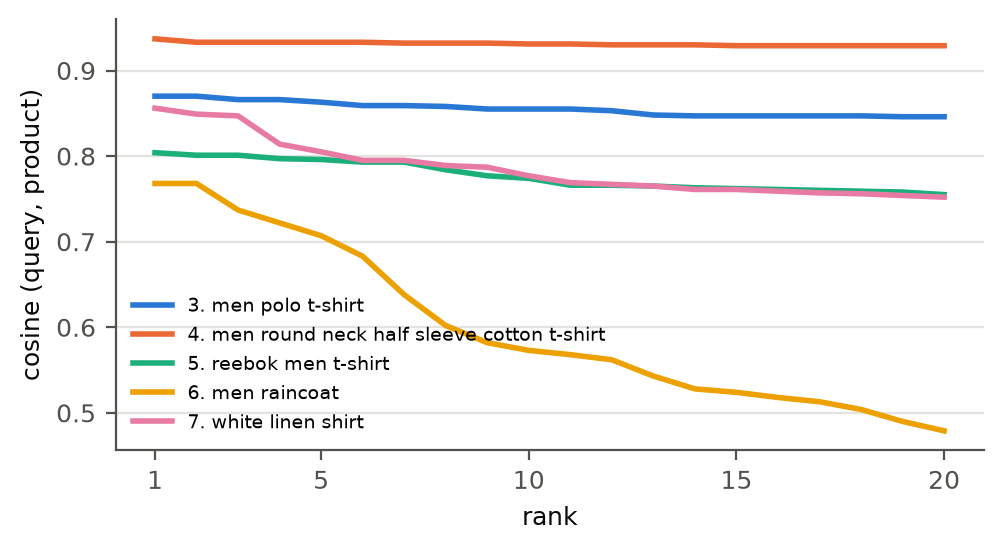
\includegraphics[width=0.72\textwidth]{word2vec_scores.png}
\caption{word2vec + cosine score against rank, top 20 of each test query. Source:
\file{word2vec\_top20.csv}.}
\label{fig:w2v}
\end{figure}

\section{A better representation than averaged word2vec}

Averaging has three problems in our data: every word counts the same (a long description drowns the
query words), word order is lost (\emph{blue jeans with white stitching} and \emph{white jeans with blue
stitching} get the same vector), and the vectors come from a small, repetitive corpus of 28,080 product
texts, one vector per word whatever its context.

\textbf{Doc2Vec} (gensim, PV-DM / PV-DBOW) learns a vector per document during training instead of
averaging afterwards. \emph{Pros:} no dilution by averaging, it captures what the product as a whole is
about, and it uses the same library. \emph{Cons:} the query is not part of training; its vector comes from
\texttt{infer\_vector}, an optimization that is noisy for 2 to 7 terms, which is exactly our case (short
queries against long products). It also has more hyper-parameters (epochs, size, mode) and changes from
run to run.

\textbf{Sentence2Vec} has two meanings. (1) \emph{SIF} (Arora et al., 2017): a weighted average where a word
weighs $a/(a+p(w))$, so frequent words count less, minus the first principal component shared by all
texts. \emph{Pros:} as cheap as our average and close in spirit to idf. \emph{Cons:} still no word order.
(2) \emph{Pretrained sentence encoders} such as Sentence-BERT (e.g.\ \texttt{all-MiniLM-L6-v2}), trained so
that texts with the same meaning get close vectors. \emph{Pros:} contextual, keep word order, handle
synonyms (\emph{sweatshirt} and \emph{hoodie}), and are trained for short queries against longer texts.
\emph{Cons:} slower (encoding 28,080 products takes minutes on a CPU instead of seconds), trained on general
English rather than fashion, harder to explain, and they need the \emph{original} text, not our stemmed
tokens without stop words. They can also blur exact attributes, ranking black jeans close to blue ones.

\textbf{Our choice: Sentence-BERT.} \reasoning{it fixes the three problems above, and its main weakness,
blurring exact attributes, matters little in our pipeline, because the AND filter already guarantees that
every candidate contains all the query words; the embedding only orders them.} A cheaper intermediate
step is a \emph{tf-idf-weighted} average of the word2vec vectors, which reuses the idf of our index and
fixes the ``every word counts the same'' problem without a new model. We did not implement either, so
this section is argued, not measured.

\section{Limitations}
\begin{itemize}
\item \textbf{Labels.} Unjudged products count as not relevant, and the test labels come from the Part 2
  ranking, so the metrics favour it (Section 1.5). Only 7 queries: differences of a few hundredths are
  noise.
\item \textbf{Parameters not tuned.} $k_1$, $b$, the factors of our score and the word2vec settings were
  set by reasoning; tuning them on these labels would inflate the evaluation.
\item \textbf{AND semantics.} A product missing one query word is never returned, whatever the ranking
  (Part 2, Section 3c). Every ranking here only reorders the same candidates.
\end{itemize}

\appendix
\section{word2vec + cosine: top 20 of the five test queries}\label{app:w2v}
\small
Source: \file{word2vec\_top20.csv}. Query ids as in the labels (3 to 7).
\subsection*{Query 3: \texttt{men polo t-shirt}}
\begin{longtable}{r r l p{0.6\textwidth}}
\toprule
Rank & Cosine & PID & Title \\
\midrule
\endhead
1 & 0.870 & \texttt{TSHFPDP66HXSHGQ9} & Typography Men Round Neck Dark Blue T-Shirt \\
2 & 0.870 & \texttt{TSHFSYGTETVWM2TZ} & Self Design Men Polo Neck Grey T-Shirt \\
3 & 0.866 & \texttt{TSHFPMSYJMYNSQMZ} & Typography Men Round Neck Black T-Shirt \\
4 & 0.866 & \texttt{TSHF98JNPUBAZYKY} & Striped Men Polo Neck Red T-Shirt \\
5 & 0.863 & \texttt{TSHFME2FSQHZVFZQ} & Tie \& Dye Men Polo Neck White, Orange, Black T-Shirt \\
6 & 0.859 & \texttt{TSHE7GY3HQGYY2JG} & Argyle Men Polo Neck Red T-Shirt \\
7 & 0.859 & \texttt{TSHFME2EDDCW37KK} & Striped Men Polo Neck White T-Shirt \\
8 & 0.858 & \texttt{TSHFME2FEYDYCXZX} & Striped Men Polo Neck Black T-Shirt \\
9 & 0.855 & \texttt{TSHFPDP6YHAYDVGZ} & Striped Men Round Neck Dark Blue T-Shirt \\
10 & 0.855 & \texttt{TSHFBU9XKCT9FZZ8} & Tie \& Dye Men Polo Neck Grey T-Shirt \\
11 & 0.855 & \texttt{TSHFME2EY4STGUPZ} & Striped Men Polo Neck White T-Shirt \\
12 & 0.853 & \texttt{TSHFXDNVQ8TUZUPF} & Striped Men Polo Neck Multicolor T-Shirt \\
13 & 0.848 & \texttt{TSHFUGKTXHZTUGCH} & Striped Men Polo Neck Blue T-Shirt \\
14 & 0.847 & \texttt{TSHFZKJHQ4GWPCDY} & Solid Men Polo Neck Grey T-Shirt \\
15 & 0.847 & \texttt{TSHFZKJHBGGUBASG} & Solid Men Polo Neck Grey T-Shirt \\
16 & 0.847 & \texttt{TSHFUGZ6GDDUVNZE} & Color Block Men Polo Neck White T-Shirt \\
17 & 0.847 & \texttt{TSHFTT2JRHHY33ZM} & Solid Men Polo Neck Multicolor T-Shirt (Pack of 4) \\
18 & 0.847 & \texttt{TSHFVUXGQU6XDFDF} & Solid Men Polo Neck White T-Shirt \\
19 & 0.846 & \texttt{TSHFTT2H7C7M8GNU} & Solid Men Polo Neck Multicolor T-Shirt (Pack of 4) \\
20 & 0.846 & \texttt{TSHFTT2KTG5KHVWP} & Solid Men Polo Neck Multicolor T-Shirt (Pack of 4) \\
\end{longtable}
\subsection*{Query 4: \texttt{men round neck half sleeve cotton t-shirt}}
\begin{longtable}{r r l p{0.6\textwidth}}
\toprule
Rank & Cosine & PID & Title \\
\midrule
\endhead
1 & 0.937 & \texttt{TSHFGZHAHVNPANGY} & Printed Men Round Neck Black T-Shirt \\
2 & 0.933 & \texttt{TSHFWMRUTHSBPXYE} & Printed Men Round Neck Yellow T-Shirt \\
3 & 0.933 & \texttt{TSHFWUDVUVV3674W} & Printed Men Round Neck White T-Shirt \\
4 & 0.933 & \texttt{TSHFGZH6ZG9YDFNJ} & Printed Men Round Neck Black T-Shirt \\
5 & 0.933 & \texttt{TSHFWQADQK6URGRN} & Printed Men Round Neck Yellow T-Shirt \\
6 & 0.933 & \texttt{TSHFGZHEQDRFWBKT} & Printed Men Round Neck Red T-Shirt \\
7 & 0.932 & \texttt{TSHFWWV7ZTEQXCPJ} & Printed Men Round Neck Green T-Shirt \\
8 & 0.932 & \texttt{TSHFWTGZGZFEFVHH} & Printed Men Round Neck Yellow T-Shirt \\
9 & 0.932 & \texttt{TSHFWWWZFWENTXMY} & Printed Men Round Neck Green T-Shirt \\
10 & 0.931 & \texttt{TSHFGZHB5WZZ4MCM} & Printed Men Round Neck Black T-Shirt \\
11 & 0.931 & \texttt{TSHFWRDATHKZFWZE} & Printed Men Round Neck Yellow T-Shirt \\
12 & 0.930 & \texttt{TSHFWRFQ3Y8FKVNE} & Printed Men Round Neck Yellow T-Shirt \\
13 & 0.930 & \texttt{TSHFGZHAEPMBH8BV} & Printed Men Round Neck Red T-Shirt \\
14 & 0.930 & \texttt{TSHFY8GTFHKVYNZR} & Printed Men Round Neck Black T-Shirt \\
15 & 0.929 & \texttt{TSHFGZKNRCNSQ64A} & Printed Men Round Neck White T-Shirt \\
16 & 0.929 & \texttt{TSHFGZKNBYBZ9FAJ} & Printed Men Round Neck Black T-Shirt \\
17 & 0.929 & \texttt{TSHFWHCEUR5GQWBN} & Printed Men Round Neck Green T-Shirt \\
18 & 0.929 & \texttt{TSHFWRFRUDQWEWGZ} & Printed Men Round Neck Green T-Shirt \\
19 & 0.929 & \texttt{TSHFWKN9FJGDY236} & Printed Men Round Neck Yellow T-Shirt \\
20 & 0.929 & \texttt{TSHFWWV7NKGXXMMP} & Printed Men Round Neck Green T-Shirt \\
\end{longtable}
\subsection*{Query 5: \texttt{reebok men t-shirt}}
\begin{longtable}{r r l p{0.6\textwidth}}
\toprule
Rank & Cosine & PID & Title \\
\midrule
\endhead
1 & 0.804 & \texttt{TSHFZ3JDHZSGCFHT} & Solid Men Round Neck Grey T-Shirt \\
2 & 0.801 & \texttt{TSHFZ3JDKTUKQF88} & Solid Men Round Neck Purple T-Shirt \\
3 & 0.801 & \texttt{TSHFGZXPFGGUCW6J} & Printed Men Round Neck Grey T-Shirt \\
4 & 0.797 & \texttt{TSHFZ3JDVAYZKCFC} & Solid Men Round Neck Grey T-Shirt \\
5 & 0.796 & \texttt{TSHFZ3JDG4PAFKYA} & Solid Men Round Neck Beige T-Shirt \\
6 & 0.793 & \texttt{TSHFK3W7SBYYGMSG} & Solid Men Round Neck White T-Shirt \\
7 & 0.793 & \texttt{TSHFGZXP87UMTGFH} & Color Block Men Round Neck Blue T-Shirt \\
8 & 0.784 & \texttt{TSHFDT66KCJEBWHF} & Solid Men Round Neck Blue T-Shirt \\
9 & 0.777 & \texttt{TSHFZ3JDWYPC2NHT} & Self Design Men Round Neck Maroon T-Shirt \\
10 & 0.774 & \texttt{TSHFZ3JDFM9YTJSC} & Self Design Men Round Neck Grey T-Shirt \\
11 & 0.766 & \texttt{TSHFCYP7WGESNMSZ} & Printed Men Round or Crew Black T-Shirt \\
12 & 0.766 & \texttt{TSHFZ3JDVXAYBQJH} & Self Design Men Round Neck Grey T-Shirt \\
13 & 0.765 & \texttt{TSHFCYPACFBXUZWZ} & Applique Men Round or Crew Grey T-Shirt \\
14 & 0.763 & \texttt{TSHFCYP7VA4YG6ZX} & Color Block Men Round or Crew Purple, White, Grey T-Shirt \\
15 & 0.762 & \texttt{TSHFDT66HBJYY4SV} & Solid Men Round Neck Blue T-Shirt \\
16 & 0.761 & \texttt{TSHFGZXQY2HPK5SB} & Self Design Men Polo Neck Black T-Shirt \\
17 & 0.760 & \texttt{TSHFZ3JDZETJHQSR} & Self Design Men Round Neck Blue T-Shirt \\
18 & 0.759 & \texttt{TSHFDT66TGFETFHR} & Solid Men Round Neck Black, Grey T-Shirt \\
19 & 0.758 & \texttt{TSHFDT66GDGHY5GK} & Solid Men Round Neck Black T-Shirt \\
20 & 0.755 & \texttt{TSHFVEV35ES5DYCY} & Sports Men Polo Neck Grey T-Shirt \\
\end{longtable}
\subsection*{Query 6: \texttt{men raincoat}}
\begin{longtable}{r r l p{0.6\textwidth}}
\toprule
Rank & Cosine & PID & Title \\
\midrule
\endhead
1 & 0.768 & \texttt{RNCF4YV4GZRYJY3A} & Solid Men Raincoat \\
2 & 0.768 & \texttt{RNCF4BYMQD53WHSF} & Solid Men Raincoat \\
3 & 0.737 & \texttt{RNCEAJYT52EVHB75} & Solid Men Raincoat \\
4 & 0.722 & \texttt{RNCEGHQUQSGXYTPD} & Solid Men Raincoat \\
5 & 0.707 & \texttt{RNCFXRFSHREUUZCN} & Solid Men Raincoat \\
6 & 0.683 & \texttt{RNCETDF8F7K5HMP3} & Solid Men Raincoat \\
7 & 0.638 & \texttt{RNCFWHY4GZDVCKWT} & Solid Men Raincoat \\
8 & 0.602 & \texttt{RNCFWZVGXMGUQDXW} & Solid Men Raincoat \\
9 & 0.582 & \texttt{RNCFGGTR5JWV8ES9} & Solid Men Raincoat \\
10 & 0.573 & \texttt{RNCFYMZ6AKKHRJC4} & Solid Men Raincoat \\
11 & 0.568 & \texttt{RNCFPBZEYAYH2HVZ} & Solid Men Raincoat \\
12 & 0.562 & \texttt{RNCFG4PHHGHSA3YH} & Solid Men Raincoat \\
13 & 0.543 & \texttt{RNCFQH2EWKYGFFFG} & Solid Men Raincoat \\
14 & 0.528 & \texttt{RNCE7YYYXTR3YD68} & Newenglandpatriots Covered From Gusty Weather Reverseable Solid Men Raincoat \\
15 & 0.524 & \texttt{RNCFT93XGKXHBHYJ} & Solid Men Raincoat \\
16 & 0.518 & \texttt{RNCFQH2EFDZZBSQD} & Solid Men Raincoat \\
17 & 0.513 & \texttt{RNCFQH2EYEMJZVVG} & Solid Men Raincoat \\
18 & 0.504 & \texttt{RNCE7A3XXRYZV25F} & Galaxy Reverseable Impenetrable Moisture Barrier Solid Men Raincoat \\
19 & 0.490 & \texttt{RNCFTPBHGZYYDHC7} & Solid Men Raincoat \\
20 & 0.479 & \texttt{RNCF75ECW2KSKEZW} & Solid Men Raincoat \\
\end{longtable}
\subsection*{Query 7: \texttt{white linen shirt}}
\begin{longtable}{r r l p{0.6\textwidth}}
\toprule
Rank & Cosine & PID & Title \\
\midrule
\endhead
1 & 0.856 & \texttt{SHTFSH5VRDYPSGGK} & Women Regular Fit Checkered Casual Shirt \\
2 & 0.849 & \texttt{SHTFSH5VCM3ZB7JC} & Women Slim Fit Checkered Casual Shirt \\
3 & 0.847 & \texttt{SHTFW9RHGPJ9QWD6} & Women Regular Fit Printed Spread Collar Formal Shirt \\
4 & 0.814 & \texttt{SHTFWAP7GH6TUU7F} & Men Regular Fit Printed Button Down Collar Casual Shirt \\
5 & 0.805 & \texttt{SHTFZZFEJJFHS3Z5} & Women Slim Fit Solid Spread Collar Formal Shirt \\
6 & 0.795 & \texttt{SHTFS2GMZSRZGM5W} & Men Slim Fit Printed Casual Shirt \\
7 & 0.795 & \texttt{SHTFS2GMNEQEGA9C} & Women Slim Fit Printed Casual Shirt \\
8 & 0.789 & \texttt{SHTEYFZAWQGZ2PPZ} & Women Regular Fit Solid Mandarin Collar Casual Shirt \\
9 & 0.787 & \texttt{SHTFS2GZVGWEWBEN} & Women Regular Fit Printed Slim Collar Casual Shirt \\
10 & 0.777 & \texttt{SHTFEKRXZHHHMSCS} & Men Slim Fit Self Design Mandarin Collar Casual Shirt \\
11 & 0.769 & \texttt{SHTFP8H9XZKAFBDF} & Women Regular Fit Checkered Formal Shirt \\
12 & 0.767 & \texttt{SHTFZ9XBC8RMRZHA} & Women Slim Fit Polka Print Casual Shirt \\
13 & 0.765 & \texttt{SHTFG3GFQAJ9YSQK} & Women Regular Fit Checkered Casual Shirt \\
14 & 0.761 & \texttt{SHTF4NAXYUN8ZT5B} & Women Slim Fit Solid Spread Collar Casual Shirt \\
15 & 0.761 & \texttt{SHTFGYHEWBFYCBXD} & Women Regular Fit Checkered Casual Shirt \\
16 & 0.759 & \texttt{SHTFCDSHVKMUUZ6V} & Men Slim Fit Solid Spread Collar Casual Shirt \\
17 & 0.757 & \texttt{SHTFM3FTBU5HWFY9} & Women Slim Fit Self Design Casual Shirt \\
18 & 0.756 & \texttt{SHTFFYF9EHF7R3W6} & Women Slim Fit Solid Spread Collar Casual Shirt \\
19 & 0.754 & \texttt{SHTFG7FMWDDNYFEY} & Women Regular Fit Printed Spread Collar Casual Shirt \\
20 & 0.752 & \texttt{SHTFM32Z3JK3YS65} & Men Slim Fit Printed Cut Away Collar Casual Shirt \\
\end{longtable}

\end{document}
